\documentclass[10pt]{article}
\usepackage{pdfpages}
\usepackage{enumitem}
\usepackage{multirow}
\usepackage[latin1]{inputenc}
\usepackage{tikz}
\usetikzlibrary{shapes, arrows}

\title{\textbf{DASH} \\Documentation}
\date{January 22, 2015}
\author{Zachary Pierson}

\begin{document}
\maketitle

\newpage
\tableofcontents
\newpage

\section{Introduction}
\paragraph{}
The c program dash is a result of the Computer Science Course 456, Operating Systems. The purpose of assignment 2 is to introduce fork and exec commands as well as pipes and redirects.  The basic approach for this program is to fork of a process and have the child execute the command via the exec. Signals are also implemented. The kill system call allows the program to send signals to other processes. dash is also able to catch signals that are sent to it.


\subsection{Description of Program}
\subparagraph{}
Not only is dash a process identification program, it is also an imitation of the bash shell. It allows the user to find process id's based on a command string, and find command strings based on process id's. dash is also capable of providing the user with process information. The second version of this project includes forks, pipes, redirects, and signals to call system calls similar to what the bash shell does.

Once invoked, dash will enter an event loop awaiting user input. Acceptable command options can be found in Table \ref{table:dashcmds} on page \pageref{table:dashcmds}.

\begin{table}[b]
\centering
\begin{tabular}{l|l}
	Command & Description\\\hline
	\textbf{cmdnm} & finds command string based on given pid\\
	\textbf{pid} & finds pid based on given command string\\
	\textbf{systat} & process information dump\\
	\textbf{help} & prints information on available commands\\
	\textbf{exit/quit} & exits the program\\
	\textbf{proc\_status} & prints process status\\
	\textbf{cd} & changes the current working directory\\
	\textbf{redirect\_pipe} & finds redirects or pipes in the input\\
	\textbf{redirected\_output} & redirects standard output to given file\\
	\textbf{redirected\_input} & redirects standard input to a file\\
	\textbf{do\_pipe} & pipes output of one command to the input of another\\
	\textbf{signal} & sends given signal to given process\\
\end{tabular}
\caption{dash commands}
\label{table:dashcmds}
\end{table}

\subsection{Compiling Instructions}
\subparagraph{}
The file can be found on github at:  https://github.com/zjpierson/operatingSystems/prog2
The Makefile supplied in the git repository is set up to compile the program into an executable called dash. This can be achived simply by typing \texttt{make} on the command line. To compile using gcc on the command line:
\begin{center}
	\texttt{gcc -o dash dash.c cmdArgs.c}
\end{center}

\subsection{Using Dash}
\subparagraph{}
First you must run the executable. This will automatically start the dash command prompt. You will then be able to use the available commands as seen in Table \ref{table:dashcmds} on page \pageref{table:dashcmds} for information on processes.\\\\
\texttt{user@host\$ ./dash\\
		dash>}

\newpage

The \texttt{cmdnm} command has an optional \texttt{[pid]} argument for finding the command string. If no arguments are passed, dash will return a list of all command strings.  An example of it use is below.\\\\
\texttt
{
dash> cmdnm 1\\
systemd\\
dash> cmdnm\\
Please specify pid. Here is a list of all cmd names:\\
systemd\,\,\,\, kthreadd\,\,\,\,\,\, ksoftirqd/0\\
rcuos/0\,\,\,\, bioset\,\,\,\,\,\,\,\,\,\,\,\, ksmd\\
crond\,\,\,\,\,\,\,\,\, watchdog/3\, bash\\
dash
}\\

The \texttt{pid} command is practically a mirror image of the \texttt{cmdnm} command. It takes an optional command string argument \texttt{[cmdnm]} and returns a list of all pid's that has a matching substring with the \texttt{[cmdnm]} argument. If no arguments are passed, dash will retun a list of all process id's. An example of its use is below.\\\\
\texttt
{
dash> pid systemd\\
1\\
dash> pid\\
Please specify cmd name. Here is a list of all pid's:\\
1\,\,\,\, 2\,\,\,\, 3\,\,\,\, 5\\
7\,\,\,\, 8\,\,\,\, 9\,\,\,\, 10\\
11\,\,12\,\, 13\\
14
}\\

The \texttt{systat} command prints diagnostic information about the process. There is no argument call to this function. The following information is what \texttt{systat} will return:

\begin{enumerate}[noitemsep]
	\item Linux Version
	\item System Uptime
	\item Total Memory
	\item Free Memory
	\item CPU information
	\item Cache size
\end{enumerate}
\hfill

The \texttt{help} command displays usage information about the program and possible arguments for the command prompt. Finally the next two commands \texttt{quit} and \texttt{exit} terminates the program and can be used interchangeably. In fact they do \textbf{exactly} the same thing as they call the same function.
\newpage

\subsection{Libraries Used}
\subparagraph{}
\begin{table}[t]
\centering
\begin{tabular}{l|c}
	Libraries & Functions Used\\\hline\hline
	\multirow{2}{*}{$<$stdio.h$>$} 
		& \texttt{fopen(), fclose(), fscanf()}\\
	 & \texttt{printf(),fgets()}\\\hline
	\multirow{2}{*}{$<$string.h$>$}
	 & \texttt{strcpy(), strcat(), strcmp(), strch()}\\
		& \texttt{strspn(), strstr(), strtok(), strlen()}\\\hline
	$<$stdlib.h$>$ & \texttt{exit()}\\\hline
	$<$dirent.h$>$ & \texttt{opendir(), readdir(), closedir()}\\
\end{tabular}
\caption{Library Functions}
\label{table:libfuncs}
\end{table}

As Illustrated in Table \ref{table:libfuncs}, the included libraries provide the program with useful functions. The  \texttt{$<$stdio.h$>$} library provides standard input output functionality to communicate with the user. These functions are scattered everywhere within the program code.

The \texttt{$<$string.h$>$} library is used for string manipulation. This library has the most diverse use of its functions mainly because there is a lot of string parsing that happens within the proc filesystem in order to retrieve process information.

The \texttt{$<$stdlib.h$>$} library is included solely for one purpose; to allow the quit function to exit the dash process when called on the command prompt. This library is not essential because there are other ways to quit the program.

The \texttt{$<$dirent.h$>$} library is used to find all directory names within /proc. This is especially useful when the pid of a command string is unknown and we have to look in every process directory to find the matching command string.

The \texttt{$<$sys/time.h$>$} and \texttt{$<$sys/resource.h$>$} libraries are used to mainly to provide process information using the \texttt{getrusage} function.

The \texttt{$<$unistd.h$>$} library allows the program to \texttt{fork} off different processes and make system calls using \texttt{execvp}. It is also used to change the current working directory by using the \texttt{chdir} function.

The \texttt{$<$fcntl.h$>$} library is used solely for the use of the \texttt{O\_RDONLY} for opening a read only file for redirected output. 

\subsection{Program Structure}
\label{subsection:structure}
\subparagraph{}
The program is broken up into 3 separate files: dash.c, cmdArgs.c, and cmdArgs.h. A structure that is important to note is the array of function pointers declared externally in cmdArgs.h and defined in cmdArgs.c. That array is closely used with the commands array declared externally in cmdArgs.h and defined in cmdArgs.c. These two arrays are used together in the \texttt{call} function to be able to invoke the correct function. Section \ref{section:algorithms} will cover this more in depth. Below is the file structure.\\

\fbox{
	\begin{minipage}{17mm}
	\centering
	\begin{small}
	cmdArgs.c
	\end{small}
	\begin{scriptsize}
	quit()\\
	cmdnm()\\
	pid()\\
	systat()\\
	help()\\
	display()\\
	\end{scriptsize}
		\hfill\vspace{3mm}
	\end{minipage} 
	}
	\hspace{5mm}
\fbox{
	\begin{minipage}{17mm}
	\centering
	\begin{small}
	cmdArgs.h
	\end{small}
	\begin{scriptsize}
		libraries\\
		\#defines\\
		prototypes\\
	\end{scriptsize}	
		\hfill\vspace{10mm}
	\end{minipage} 
	}
	\hspace{5mm}
\fbox{
	\begin{minipage}{17mm}
	\centering
	\begin{small}
	dash.c
	\end{small}
	\begin{scriptsize}
	main()\\
	\end{scriptsize}
		\hfill\vspace{15mm}
	\end{minipage} 
	}

\section{Algorithms}
\label{section:algorithms}
\paragraph{}
As briefly mentioned in Section \ref{subsection:structure}, there is an array of function pointers used in \texttt{call} to invoke the appropriate function. For modularity sake, the \texttt{\#define NUM\_CMDS} is used to keep track of the number of commands the user can enter. To add another command, one would simply increase \texttt{NUM\_CMDS} and add the function to both the \texttt{commands} array and the \texttt{func} array. Obviously the function would need to be declared in cmdArgs.h and defined in cmdArgs.c as well.

\subsection{Event Loop}
\label{section:eventLoop}
\subparagraph{}
As stated before in both Sections \ref{subsection:structure} \& \ref{section:algorithms}, the \texttt{call} function makes use of function pointers to call the appropriate method. The \texttt{main()} function in dash.c contains and handles the event loop. Figure \ref{figure:main} demonstrates the structure.

% Define block styles
\tikzstyle{decision} = [diamond, draw, fill=blue!20, 
    text width=4.5em, text badly centered, node distance=3cm, inner sep=0pt]
\tikzstyle{block} = [rectangle, draw, fill=blue!20, 
    text width=5em, text centered, rounded corners, minimum height=4em]
\tikzstyle{line} = [draw, -latex']
\tikzstyle{cloud} = [draw, ellipse,fill=red!20, node distance=3cm,
    minimum height=2em]

\begin{center} 
\begin{figure}
\begin{tikzpicture}[node distance = 2cm, auto]
\begin{small}

\node[cloud](start)
	{Start};
\node[block, right of = start, node distance=3cm](while)
	{Enter \texttt{while(1)} loop};
\node[block, right of = while, node distance=3cm](prompt)
	{Display \texttt{dash>} prompt};
\node[decision, below of = while, text width=7em](validInput)			{Input only contains white space};
\node[block, left of = validInput, node distance=4cm, text width=7em](extract)
	{extract the first word (cmd) using \texttt{strtok()}};
\node[block, below of = extract, text width=7em, node distance=4cm](commandLoop)
	{Loop though all valid commands};
\node[decision, right of = commandLoop, text width = 8em, node distance=4cm](cmp)
	{\texttt{cmd$=$command[i]}?};
\node[block, right of = cmp, node distance=4.5cm, text width=10em](call)
	{Call function:\\ \texttt{(*func[i])(input)} };
\node[block, below of = commandLoop](increment)
	{increment \texttt{i}};
	
\path[line](start)--(while);
\path[line](while)--(prompt);
\path[line](prompt)--(validInput);
\path[line](validInput)-| node[near start] {Yes}(prompt);
\path[line](validInput)-- node[near start] {No}(extract);
\path[line](extract)--(commandLoop);
\path[line](commandLoop)--(cmp);
\path[line](cmp)-- node[near start] {Yes}(call);
\path[line](cmp)|- node[near end] {No}(increment);
\path[line](increment)--(commandLoop);
	
\end{small}	
\end{tikzpicture}
\vspace{5mm}
\centering
\caption{\texttt{call} function}
\label{figure:main}
\end{figure}
\end{center}

\subsection{Functions}
\subparagraph{}
The purpose of this section is to describe the algorithms for each of the commands that dash supports. A list of possible commands can be found in Table \ref{table:dashcmds} on page \pageref{table:dashcmds}. 


\subsubsection{cmdnm}
\subparagraph{}
The function \texttt{cmdnm()} first checks if an argument was passed. White space does not count as an argument and therefore calls another function \texttt{display\_cmdNames()} which displays all command strings. If an argument is passed, then \texttt{cmdnm()} will attempt to open the file \texttt{/proc/$<$pid$>$/comm}. On success, the contents of the file will be displayed to the user (The \texttt{/comm} file contains the command string). Figure \ref{figure:cmdnm} on page \pageref{figure:cmdnm} is a flowchart of the algorithm used.

\begin{figure}
\centering
\begin{tikzpicture}[node distance=2cm, auto]
\begin{small}


\node[cloud](start)
	{cmdnm()};
\node[decision, below of = start, node distance=2.5cm](argument)
	{Specifyed argument for \texttt{cmdnm}?};
\node[block, left of = argument, node distance=4cm](Arg)
	{Argument specifyed};
%No arguments supplied
\node[block, right of = argument, node distance=4cm](noArg)
	{Diaplay all possible command strings};
\node[cloud, below of = noArg, node distance=2.5cm](displayCMD)
	{\texttt{display\_cmdNames()}};
\node[block, below of = displayCMD, text width=7em](dirLoop)
	{Loop though all directory names in \texttt{/proc}};
\node[decision, below of = dirLoop](isNumber)
	{Is this directory a number};
\node[decision, left of = isNumber, text width=3em, node distance=2.5cm](more)
	{More?};
\node[block, below of = isNumber, text width=9em, node distance=3cm](print)
	{Print contnets of \texttt{/proc/<pid>/comm}};
%Arguments supplied
\node[decision, below of = Arg](open)
	{Try opening given file};
\node[block, right of = open, minimum height=2em, node distance=4cm](error)
	{Print error};
\node[cloud, below of = error, node distance=3cm](return)
	{Return};
\node[block, below of = open, text width=9em, node distance=3cm](comm)
	{read and print from: \texttt{/proc/$<$pid$>$/comm}};


\path[line](start)--(argument);
\path[line](argument)-- node[near start]{No}(noArg);
\path[line](argument)-- node[near start]{Yes}(Arg);
%No arguments supplied
\path[line, dashed](noArg)--(displayCMD);
\path[line](displayCMD)--(dirLoop);
\path[line](dirLoop)--(isNumber);
\path[line](isNumber)-- node[near start]{No}(more);
\path[line](more)|- node[near start]{Yes}(dirLoop);
\path[line](isNumber)-- node[near start]{Yes}(print);
\path[line](more)-| node[near start]{No}(return);
%Arguments supplied
\path[line](Arg)--(open);
\path[line](open)-- node[near start]{Failed}(error);
\path[line](error)--(return);
\path[line](open)-- node[near start]{Successful}(comm);
\path[line](comm)--(return);
\path[line](print)-|(more);

\end{small}
\end{tikzpicture}
\vspace{5mm}
\caption{The \texttt{cmdnm} function}
\label{figure:cmdnm}
\end{figure}


\subsubsection{pid}
\subparagraph{}
The function \texttt{pid()} first checks if an argument was passed, similar to \texttt{cmdnm()}. White space does not count as an argument and therefore calls another function \texttt{display\_pid()} which displays all the process ids. If an argument is passed, then \texttt{pid()} enters a loop that goes though every process directory in \texttt{/proc}. In this manner, every process's \texttt{comm} file will be opened and checked for substring matches with the argument. All processes that match a substring will be displayed for the user. Figure \ref{figure:pid} on page \pageref{figure:pid} is a flowchart of the algorithm used.


\begin{figure}
\centering
\begin{tikzpicture}[node distance=2cm, auto]
\begin{small}

\node[cloud](start)
	{\texttt{pid()}};
\node[decision, below of = start, node distance=2.5cm](argument)
	{Specifyed argument for \texttt{pid}?};
\node[block, left of = argument, node distance=5cm, text width=7em](Arg)
	{Loop though all directory names in \texttt{/proc}};
%No arguments supplied
\node[block, right of = argument, node distance=5cm](noArg)
	{Diaplay all possible process id's};
\node[cloud, below of = noArg, node distance=2.5cm](displayCMD)
	{\texttt{display\_pid()}};
\node[block, below of = displayCMD, text width=7em](dirLoop)
	{Loop though all directory names in \texttt{/proc}};
\node[decision, below of = dirLoop](isNumber)
	{Is this directory a number};
\node[decision, left of = isNumber, text width=3em, node distance=2.5cm](more)
	{More?};
\node[block, below of = isNumber, node distance=3cm](print)
	{Print directory name};
%Arguments supplied
\node[decision, below of = Arg](argisNumber)
	{Is this directory a number};
\node[decision, right of = argisNumber, text width=3em, node distance=2.5cm](argmore)
	{More?};
\node[block, below of = argisNumber, node distance=3cm](open)
	{Open and read comm file};
\node[decision, below of = open](match)
	{Does command match substring?};
\node[cloud, below of = error, node distance=3cm](return)
	{Return};
\node[block, below of = match, text width=9em, node distance=3cm](comm)
	{Print from: \texttt{/proc/$<$pid$>$/comm}};


\path[line](start)--(argument);
\path[line](argument)-- node[near start]{No}(noArg);
\path[line](argument)-- node[near end]{Yes}(Arg);
%No arguments supplied
\path[line, dashed](noArg)--(displayCMD);
\path[line](displayCMD)--(dirLoop);
\path[line](dirLoop)--(isNumber);
\path[line](isNumber)-- node[near start]{No}(more);
\path[line](more)|- node[near start]{Yes}(dirLoop);
\path[line](isNumber)-- node[near start]{Yes}(print);
\path[line](more)-| node[near start]{No}(return);
\path[line](print)-|(more);
%Arguments supplied
\path[line](Arg)--(argisNumber);
\path[line](argisNumber)-- node[near start]{No}(argmore);
\path[line](argisNumber)-- node[near start]{Yes}(open);
\path[line](open)--(match);
\path[line](match)-| node[near start]{No}(argmore);
\path[line](match)-- node[near start]{Yes}(comm);
\path[line](comm)-|(argmore);
\path[line](argmore)|-(Arg);
\path[line](argmore)-| node[near start]{No}(return);


\end{small}
\end{tikzpicture}
\vspace{5mm}
\caption{The \texttt{pid} function}
\label{figure:pid}
\end{figure}

\subsubsection{systat}
\subparagraph{}
The \texttt{systat()} function is much simpler than the other \texttt{cmdnm()} and \texttt{pid()} functions. The Table \ref{table:procFiles} on page \pageref{table:procFiles} shows the contents of certain files that \texttt{systat()} uses. The function opens each file and extracts the information using many of the string functions that can be found in Table \ref{table:libfuncs} on page \pageref{table:libfuncs}.


\begin{table}[b]
\centering
\begin{tabular}{c|l}
	Files & Information\\\hline\hline
	\texttt{/proc/version} & Linux Version information\\
	\texttt{/proc/uptime} & System uptime\\
	\texttt{/proc/meminfo} & Total Memory, Free Memory\\
	\texttt{/proc/cpuinfo} & Vendor id though cache size\\
\end{tabular}
\vspace{2mm}
\caption{Useful process files}
\label{table:procFiles}
\end{table}


\subsubsection{exit}
\subparagraph{}
The \texttt{exit()} function is literally the sole reason why \texttt{$<$stdlib.h$>$} was included, for the use of it's exit() command.


\subsubsection{cd}
\subparagraph{}
The \texttt{cd()} function is much simpler than many of the other functions. This one simply makes a call to \texttt{chdir()} which changes the current working directory. 

\newpage

\subsubsection{signal}
\subparagraph{}
The \texttt{signal} command is used to send signals to other processes. This function is basically a wrapper for the \texttt{kill} system call. A new variable called \texttt{cmd} is used as the actual argument to \texttt{execvp()}. \texttt{cmd} is initialized with {"kill", "-s"} and appends the rest of the arguments from \texttt{args} to \texttt{cmd}.


\section{Testing and Verification}
\paragraph{}
All functions were tested and have passed inspections. The purpose of this section is demonstrate the testing and verification process. Multiple attempts at trying to break the program will be covered and any unwanted behavior will be reported in this section.


\subsection{Event Loop}
\subparagraph{}
The Event loop was thoroughly tested. No amount of white spaces or random characters seems to crash the program. Error messages are robust and include detailed information on what failed and how to use dash correctly.  The event loop was tested and passed all inspections.

\subsection{cmdnm}
\subparagraph{}
As with the event loop, no amount of white spaces or random characters seems to crash the program. The main concern with the \texttt{cmdnm()} function was weather a non-process id directory would crash the program. However, other directories such as \texttt{bus} and \texttt{driver} when passed to \texttt{cmdnm()} does not crash the program. Any additional arguments to this function will be ignored.

\subsection{pid}
\subparagraph{}
As with the other functions, no amount of white spaces or random characters seems to crash the program. There were not many concerns about this function and is proving to be accurate and robust. Any additional arguments to this function will be ignored.

\subsection{systat}
\subparagraph{}
There was not many test cases to run on the \texttt{systat()} function. The output of this function matches the actual system process information gathered from \texttt{ps}. Like the other functions, any additional arguments supplied to \texttt{systat()} will be ignored. 

\subsection{cd}
\subparagraph{}
Initially, when the \texttt{cd} function was implemented, it seemed as if it had not changed the current working directory. However, on latter attempts It was found that once the child process had terminated, the \texttt{chdir} no longer contained the correct directory. The solution to this was to call the \texttt{cd} command directly in the Event Loop.

\subsection{signal}
\subparagraph{}
Not only can dash send specific signals to processes, but it can also catch any signal except for \texttt{SIGKILL} and \texttt{SIGSTOP}. Many tests were done and it is concluded that the signal command is properly functioning.

\subsection{pipes and redirected input/output}
\subparagraph{}
This is an important section to include here as it is  not fully satisfying. First of all, the symbols "\texttt{<>|}" need to be surrounded by white space for dash to recognize their meaning. Secondly, the pipes take 2 commands that get piped together. This is a problem when the user wishes to pipe more than two commands together. A note in the program documentation explains that these are to be implemented in the future. Other than that, these features work great and hold up many different test cases.

\subsection{exit}
\subparagraph{}
The \texttt{exit()} function does exit the program and therefore works as expected. This function passes inspection.


\section{Description of Submission}
\paragraph{}
The submission of this program will consist of the following items within \texttt{prog1.tgz} file.

\begin{enumerate}[noitemsep]
\item prog2.pdf
\item dash.c
\item cmdArgs.c
\item cmdArgs.h
\item Makefile
\end{enumerate}

\vfill
\section{APPENDICES}
\appendix

\section{Program Assignment}
%\label{App:AppendixA}
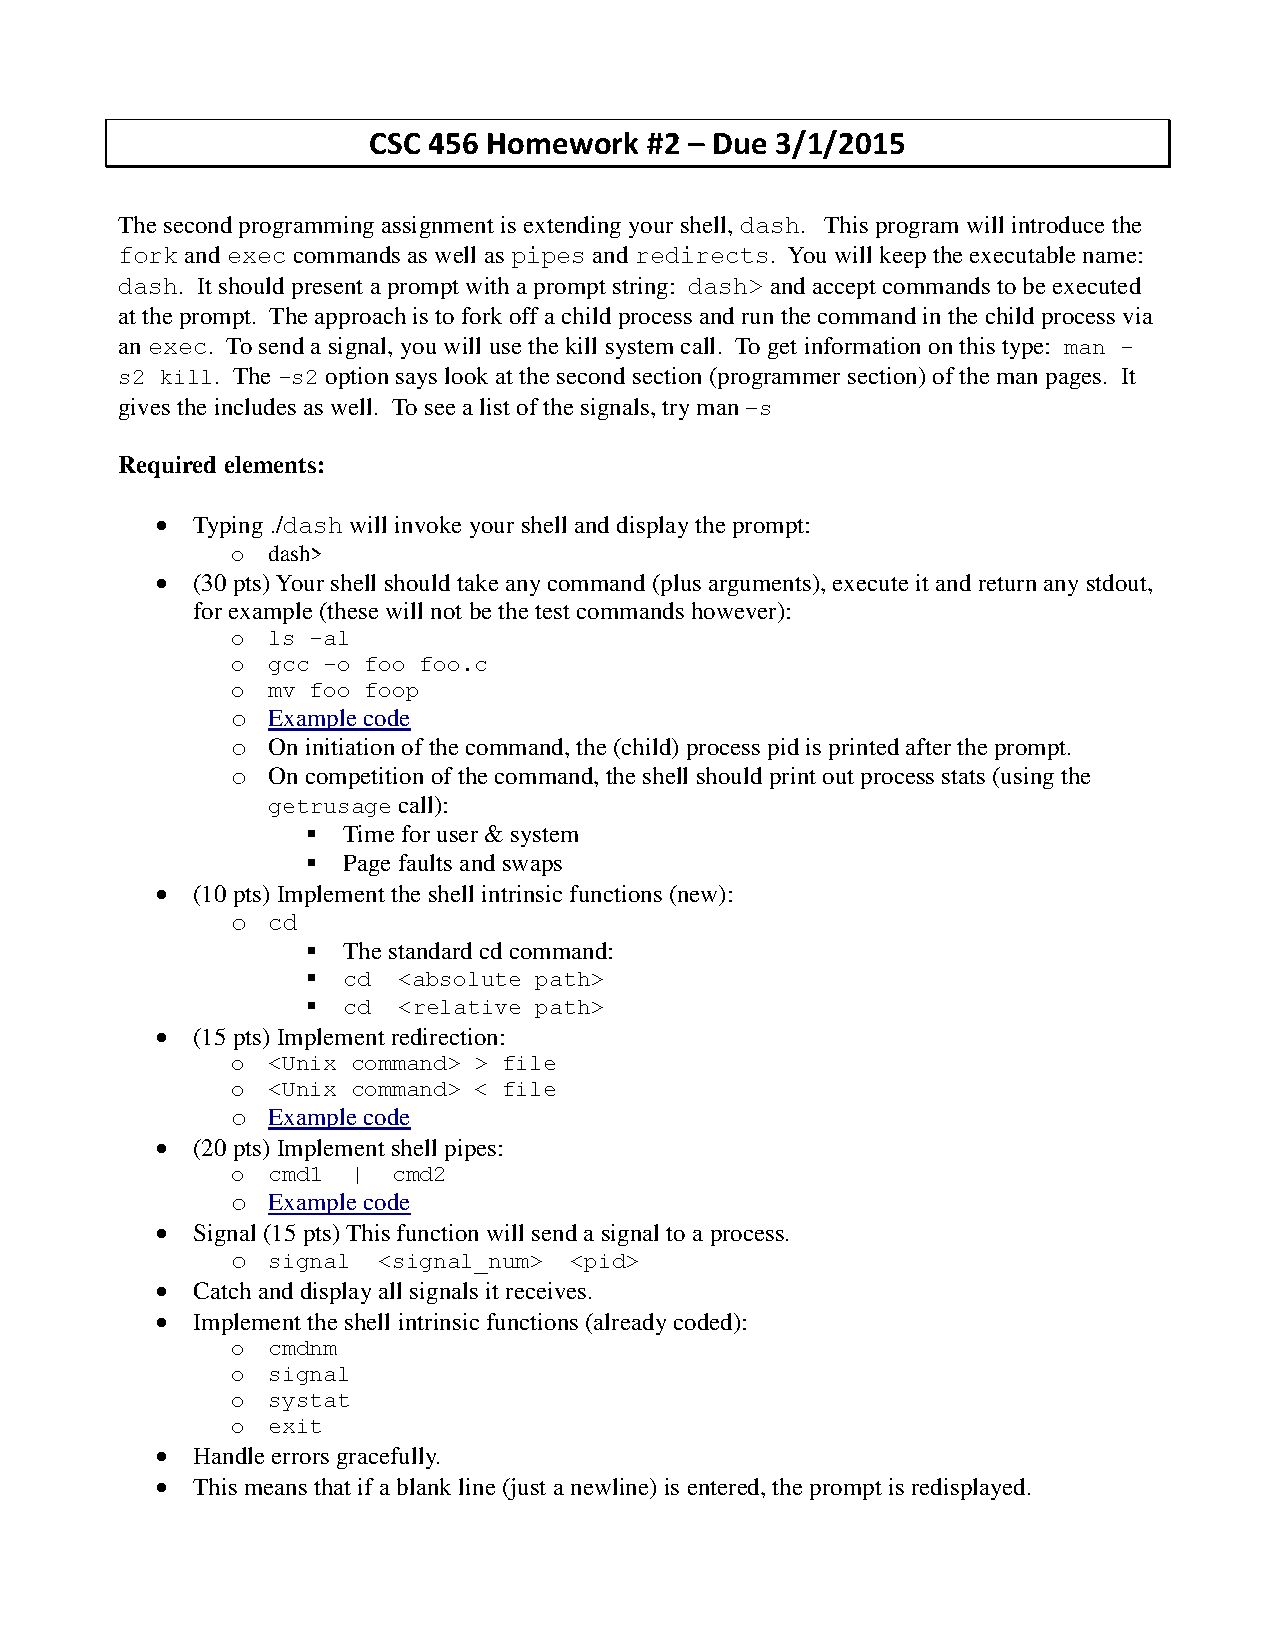
\includepdf[pages={1-4},frame={true}]{csc456_HW2.pdf}


\end{document}